% Live measurements only. Derived figures and aggregates retain the sealed
% September 25 evidence hashes; simulator results are not pooled with this pair.
\subsubsection{Native TTL During Two Delivery Bursts}
\label{sec:ttl-loaded-results}

Before the preload trial, a separate live pair tested native TTL against a
static TTL-disabled control on one isolated Oracle Cloud subscriber Pod.
Both arms used 5,000 subscriptions, five clients, 20 occupied connections and
five empty probes, with zero artificial client processing delay. Each started
from an empty Queue and received two bursts of three accepted source events,
giving 30,000 recorded delivery attempts per arm. Both used the same server
image and 900-second post-activation observation. Native TTL retained its
original jitter. The control replayed the accepted burst schedule: its first
requests were 0.462 and 0.578 seconds later than the native relative targets
of 26.182 and 319.207 seconds. Queue-statistics budget failures stopped other
publication blocks before any event attempt; those failures were retained.

\begin{table}[!htbp]
 \centering
 \small
 \renewcommand{\arraystretch}{1.14}
 \caption{Oracle Cloud two-burst TTL comparison, separate from the subsequent
 preload pair. Both arms use static placement on one Pod; TTL off is not a
 learned DQL intervention. Latency statistics include confirmed ACKs only.}
 \Description{Native TTL records five interruptions, 369 unresolved receipts
 and a 238.392-second confirmed ACK latency p95. The static TTL-disabled control
 records zero interruptions, no unresolved receipts and a 55.826-second p95.}
 \label{tab:ttl-loaded-results}
 \begin{tabular}{p{0.51\linewidth}rr}
  \toprule
  Measurement & Native TTL & Static TTL off \\
  \midrule
  Delivery attempts & 30,000 & 30,000 \\
  Receipt-confirmed ACKs & 29,631 & 30,000 \\
  Unresolved ACK receipts & 369 & 0 \\
  Server-matched TTL interruptions & 5 & 0 \\
  Confirmed ACK latency: median (s) & 19.439 & 21.407 \\
  Confirmed ACK latency: 95th percentile (s) & 238.392 & 55.826 \\
  Clients with receipt-complete shutdown & 2 of 5 & 5 of 5 \\
  \bottomrule
 \end{tabular}
\end{table}

Table~\ref{tab:ttl-loaded-results} shows the tail that a median alone would
miss: native TTL's confirmed-ACK p95 was 4.27 times the control's, although its
median was 1.968 seconds lower. Five interruptions matched server expiry records.
Transport reconnection took 17--24~ms, whereas restoring all 250 bindings on
each affected connection took 0.504--0.973 seconds. One recovery received
22 delivery callbacks before all binding receipts arrived. This directly
demonstrates delivery overlapping resubscription within the observed short
recovery windows; prolonged stalls and whole-pool expiry were not observed. All 369 unresolved
attempts belonged to expired sessions; three clients reached the 120-second
receipt-drain deadline. Missing receipts are not counted as lost Queue events.
All ten sealed client bundles were recovered and verified. This single
sequential pair measures TTL-related disruption and confirmed-receipt latency
under static placement. It estimates neither repeated-run capacity nor a
DQL-specific effect.

\subsubsection{Matched-Preload Comparison in the Oracle Cloud Cluster}
\label{sec:ttl-preload-results}

A subsequent isolated trial compared native TTL with the frozen DQL controller
under the same initial queued workload. Each arm used the same 5,000 registered
ET1 subscriptions: five clients held 1,000 subscriptions each on four occupied
connections, with 250 subscriptions per connection and one empty probe per
client. All 20 occupied connections initially terminated on one subscriber Pod.
Three identical Pods became Ready before activation. Each Pod had a limit of
three CPU cores and 6~GiB memory, and both arms used the same pinned server image.
The installed Queue limit remained 400,000,000 bytes; shared subscriber
resources were not changed.

All bindings were attached in standby before six source events were published
through the authenticated ingest path. A pre-activation Queue snapshot verified
30,000 visible copies and zero in-flight copies in each arm. The recorded
delivery ledger subsequently contained six attempts for every subscription in
the same 5,000-subscription cohort. Native TTL retained the 60-second base,
1--60-minute random jitter and scheduled scan. The DQL arm disabled TTL and
loaded unchanged online and target networks from the checkpoint with 9,985
training updates; exploration and further learning were disabled. Observation
continued for 900 seconds after activation, with activation itself also recorded.

The original workload included a six-event refill at five minutes. Its first
Queue-statistics budget check returned HTTP~429 before any event was attempted.
Before the DQL arm started, the comparison was amended to use the six-event
preload without refill. Three DQL preload budget checks also failed before
publication; cooldown and fresh checks admitted the remaining events while all
bindings stayed in standby. The initial copy counts therefore matched, but the setup proceeded at
different rates. Queue occupancy was approximately 20.3~MB in both arms, not
400~MB. This sequential pair measures fixed-preload drainage. Sustained
arrivals and subscriber saturation are outside that workload.

\subsubsection{Receipt Completion and Connection Recovery}

Table~\ref{tab:ttl-preload-results} reports the observed outcomes. Let
$D_{\mathrm{obs}}$ be the number of recorded delivery attempts and
$A_{\mathrm{conf}}$ the number with a confirmed ACK receipt. Receipt completion is
$A_{\mathrm{conf}}/D_{\mathrm{obs}}$; the remainder is unresolved, not classified as
event loss. Both arms recorded 30,000 attempts. Native TTL confirmed 26,831 ACKs
(89.44\%), compared with 30,000 (100\%) in the TTL-disabled arm, a difference of
10.56 percentage points in this pair. The latter arm is labelled
\emph{guard-held DQL}: its controller ran, but telemetry guards held every
decision at \emph{stay}, as explained below.

\begin{table}[!htbp]
 \centering
 \small
 \renewcommand{\arraystretch}{1.14}
 \caption{Measured Oracle Cloud outcomes for the matched 5,000-subscription
 preload. The DQL arm had TTL disabled and executed no migration. Latencies
 are conditional on confirmed ACKs; unresolved receipts are reported separately.}
 \Description{Both arms record thirty thousand delivery attempts. Native TTL
 has twelve server-matched interruptions and 3,169 unresolved receipts. The
 guard-held DQL arm has neither, but executes no migrations.}
 \label{tab:ttl-preload-results}
 \begin{tabular}{p{0.49\linewidth}rr}
  \toprule
  Measurement & Native TTL & Guard-held DQL \\
  \midrule
  Delivery attempts & 30,000 & 30,000 \\
  Receipt-confirmed ACKs & 26,831 & 30,000 \\
  Unresolved ACK receipts & 3,169 & 0 \\
  Receipt completion (\%) & 89.44 & 100.00 \\
  Server-matched TTL interruptions & 12 & 0 \\
  Distinct occupied sockets interrupted & 11 of 20 & 0 of 20 \\
  Peak simultaneously recovering sockets & 3 of 20 & 0 of 20 \\
  Incomplete-restoration exposure (connection-s) & 10.983 & 0 \\
  Confirmed ACK latency: median (s) & 69.862 & 69.836 \\
  Confirmed ACK latency: 95th percentile (s) & 251.546 & 249.874 \\
  Executed DQL migrations & Not applicable & 0 \\
  \bottomrule
 \end{tabular}
\end{table}

All twelve native interruptions matched server expiry records by session
identity and disconnect time. They affected eleven distinct occupied sockets,
with at most four interrupted within a rolling minute. At most three sockets
were concurrently unrestored, giving $\max_s F(s)=3/20=0.15$ and
$\int\sum_c I_c(s)\,ds=10.983$ connection-seconds. Complete binding
restoration took 0.492--1.835 seconds. These observations show overlapping
recovery periods affecting part of the pool, rather than a whole-pool outage. All 3,169 unresolved native
attempts belonged to sessions with matched expiries, but a missing ACK receipt
does not reveal whether the underlying Queue deletion succeeded.

\begin{figure}[!htbp]
 \centering
 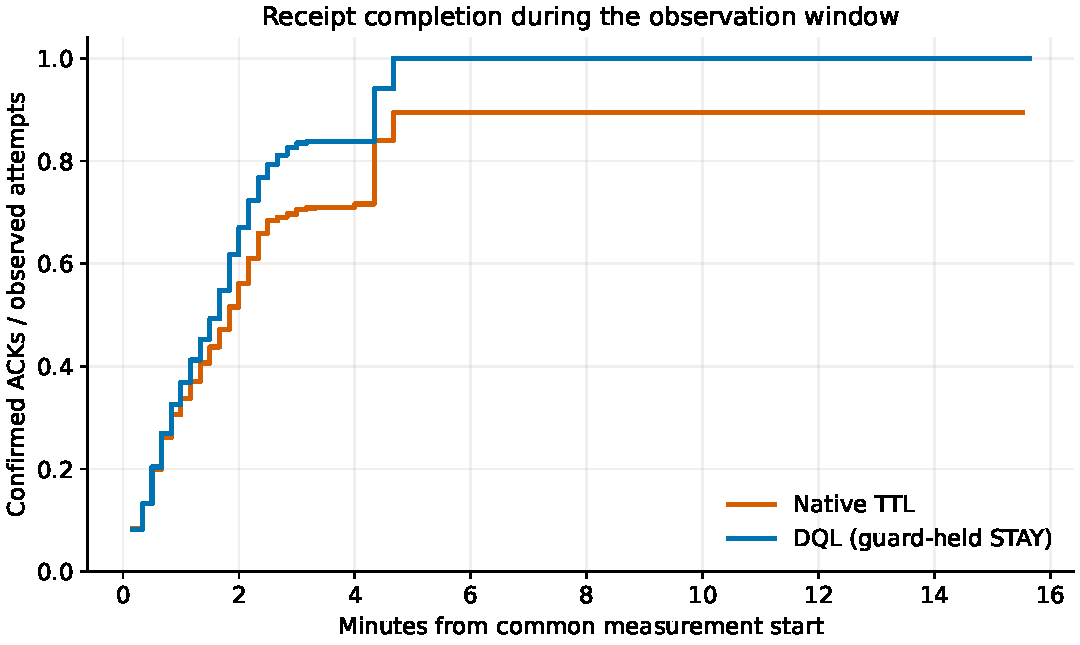
\includegraphics[width=0.88\textwidth]{figures/ttl-preload-ack-completion.pdf}
 \caption{Receipt completion in the Oracle Cloud matched-preload pair.
 Each curve accumulates confirmed ACKs in ten-second bins and divides by all
 30,000 observed attempts in its arm. Unresolved attempts remain in the
 denominator. DQL denotes the guard-held, TTL-disabled execution, not a
 completed migration comparison.}
 \Description{Native TTL receipt completion reaches 89.44 percent and the
 guard-held DQL arm reaches 100 percent. The horizontal axis is minutes from
 the common measurement start within each arm.}
 \label{fig:ttl-preload-completion}
\end{figure}

Figure~\ref{fig:ttl-preload-completion} retains the unresolved attempts in the
final level rather than rescaling each curve using only successful attempts.
Time starts when all five client observation windows overlap within each arm. Those common windows lasted 931.347 and 937.743 seconds,
respectively. Their mean confirmed-ACK rates were 28.809 and 31.992/s, including
idle time; these are whole-window completion rates, not estimates of maximum
Pod bandwidth. Four native clients reached the 120-second final ACK-drain
deadline. We retain their incomplete drains and the coordinator's nonzero exit status
as outcomes. All ten client evidence bundles were sealed and verified;
the DQL coordinator completed cleanly.

\begin{figure}[!htbp]
 \centering
 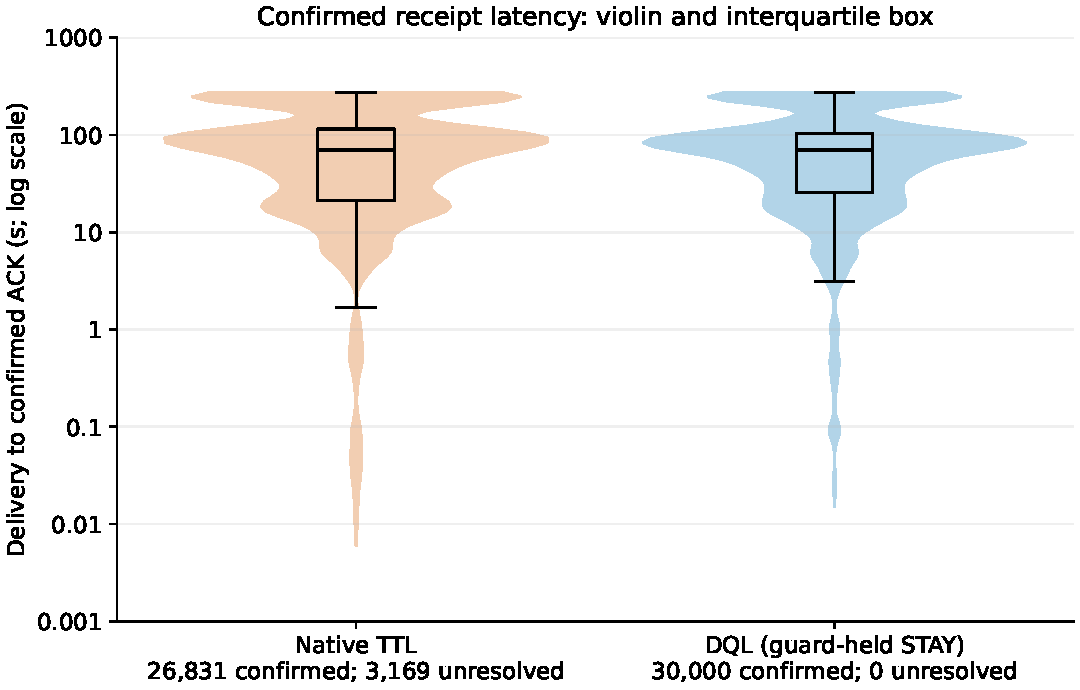
\includegraphics[width=0.88\textwidth]{figures/ttl-preload-ack-latency-violin-box.pdf}
 \caption{Confirmed delivery-to-ACK latency in the Oracle Cloud preload pair.
 Violin density is estimated on $\log_{10}$ latency; boxes show its median and
 interquartile range, with 1.5-IQR whiskers. Outlier markers are suppressed,
 not removed from the observations. Counts exclude unresolved receipts.}
 \Description{Violin and box plots compare 26,831 confirmed native TTL
 latencies with 30,000 guard-held DQL latencies. Their medians are approximately
 seventy seconds. Native TTL additionally has 3,169 unresolved receipts.}
 \label{fig:ttl-preload-latency}
\end{figure}

Figure~\ref{fig:ttl-preload-latency} separates receipt completion from
conditional latency. The confirmed medians differ
by only 0.026 seconds, and the 95th percentiles are also close. Native unresolved
receipts are absent from this latency distribution but remain explicit in
Table~\ref{tab:ttl-preload-results}. Violin width describes within-run latency
variation. The five clients and 30,000 attempts belong to one pair rather than
independent trials, so between-run uncertainty is not estimated. Unlike the
earlier 104.174-second diagnostic, this pair recorded no new delivery callbacks
during subscription-restoration windows. It captures a different recovery
condition from resubscription under concurrent delivery.

\subsubsection{Telemetry Freshness and Action Eligibility}

The DQL trace contains 450 decision intervals, all held at \emph{stay} by
\texttt{invalid-backlog-telemetry}. No migration executed, and all 5,000 bindings
remained on the source Pod despite four Pods being Ready. Statistics collection
paced individual subscription requests at 40~ms for a 5,000-subscription sweep.
Even before network delay or retries, the sweep required at least
$5{,}000\times0.040=200$ seconds, exceeding the 180-second oldest-sample deadline.
The minimum coverage across the Pod and occupied-connection components ranged
from 0.560 to 0.808. Only ten observations met every 80\% coverage threshold;
their oldest constituent samples were 183.127--185.974 seconds old and failed
freshness. A recently received telemetry frame can therefore contain stale
Queue observations. Queue-statistics rate limits further constrained coverage.

This finding separates two operational properties. Native expiry produced
measurable interruptions and receipt uncertainty; the TTL-disabled, guard-held
arm preserved its occupied sockets and completed all observed ACKs. Freshness
checks held migration inactive, so the measured benefit concerns connection
retention and receipt completion, rather than throughput from added Pod
capacity. The checkpoint and guards stayed fixed throughout the trial.
Cleanup verified empty Queue and
dead-letter Queue inventories, restored isolated TTL to zero and one Ready Pod,
and passed all thirteen shared-resource isolation checks.
\FloatBarrier
